%%%%%%%%%%%%%%%%%%%%%%%%%%%%%%%%%%%%%%%%%%%
% \documentclass[a4paper,5p, review]{elsarticle}
 \documentclass[final,5p,times,twocolumn,hyphens]{elsarticle}

\usepackage[switch, columnwise]{lineno}
\usepackage{easylist}
\usepackage{amssymb}
\usepackage{amsmath}
\usepackage{subcaption}
\usepackage[breaklinks]{hyperref}
\usepackage{url}
\usepackage{textcomp}
\usepackage{verbatim}
\usepackage[ruled,vlined]{algorithm2e}
\usepackage{ulem}
\usepackage{stfloats}
%\usepackage[ampersand]{easylist}
\setcounter{tocdepth}{3}
\usepackage{graphicx}
\usepackage{pgfplots}
\usepackage{listings}
\usepackage{enumitem}
\usepackage{wrapfig}
\hypersetup{breaklinks=true}

\DeclareMathOperator{\Rcal}{\mathcal{R}}
\newcommand{\bw}{\mathbf{w}}

\pgfplotsset{compat=1.14}
\pgfplotsset{compat=newest}
\pgfplotsset{plot coordinates/math parser=false}
\usepackage{tikzscale}
\usetikzlibrary{matrix,chains,positioning,decorations.pathreplacing,arrows}
\usepackage{tikz-qtree,tikz-qtree-compat}
\usetikzlibrary{calc}
\modulolinenumbers[5]
\usepackage[numbers]{natbib}

\usepackage{enumitem}
\usepackage{array}

\journal{Future Generation Computer Systems}

\pdfstringdefDisableCommands{%
  \def\corref#1{}%
}

%% `Elsevier LaTeX' style
\bibliographystyle{elsarticle-num-names}

\newcommand{\researchquestions}{
    \begin{enumerate}
        \item How are state-of-the-art xAI approaches interpreted and evaluated by expert users in a typical diagnostic setting?
        \item How do these interpretations and evaluations inform principles for the development of safe and effective xAI?
    \end{enumerate}
}

%%%%%%%%%%%%%%%%%%%%%%%

\begin{document}

\begin{frontmatter}

\title{The Explainability Paradox: Challenges for xAI in Digital Pathology}

%% or include affiliations in footnotes:
\author[TUB]{Theodore Evans\corref{mycorrespondingauthor}}
\cortext[mycorrespondingauthor]{Corresponding author}
\ead{theodore.evans@dai-labor.de}
\author[TUB]{Carl Orge Retzlaff}
\author[TUB]{Christian Geißler}
\author[MUG]{Michaela Kargl}
\author[MUG]{Markus Plass}
\author[MUG]{Heimo~M{\"u}ller}
\author[CAR]{Tim-Rasmus Kiehl}
\author[CAR]{Norman Zerbe}
\author[MUG]{Andreas Holzinger }

\address[TUB]{DAI-Labor, Technical University of Berlin, Germany}
\address[MUG]{Medical University Graz, Austria}
\address[CAR]{Charité – Universit{\"a}tsmedizin Berlin, corporate member of Freie Universit{\"a}t Berlin and Humboldt- Universit{\"a}t zu Berlin, Institute of Pathology, Germany}

\begin{abstract} 
The increasing prevalence of digitized workflows in diagnostic pathology opens the door to life-saving applications of artificial intelligence (AI). Explainability is identified as a critical component for the safety, approval and acceptance of AI systems for clinical use. Despite the cross-disciplinary challenge of building explainable AI (xAI), very few application- and user-centric studies in this domain have been carried out. We conducted the first mixed-methods study of user interaction with samples of state-of-the-art AI explainability techniques for digital pathology. This study reveals challenging dilemmas faced by developers of xAI solutions for medicine and proposes empirically-backed principles for their safer and more effective design.
\end{abstract}

\begin{keyword}
Explainable AI, Digital Pathology, Usability, Trust, Artificial Intelligence
\end{keyword}

\end{frontmatter}
\linenumbers

\section*{\textbf{Highlights}}

\begin{itemize}
    \item A novel study evaluating state-of-the-art xAI approaches on expert users in pathology
    \item Pathologists prefer simple, visual explanations that mirror their way of thinking
    \item Designing xAI involves difficult-to-resolve conflicts between usability and user bias
    \item Safe and effective explainability should be part of AI development from day one
    \item No explainability may be better than bad explainability
\end{itemize}

\section{Introduction}
\label{sec:introduction}

Pathology is poised at the brink of an AI renaissance. For almost two centuries, the analysis of tissue has taken place primarily through the lens of a microscope. In the past decade, the proliferation of digitized workflows has intersected with a dramatic rise in machine learning (ML) capabilities~\cite{Pantanowitz:2010:DigitalPathology,PantanowitzEtAl:2021:AIPatho}, promising improved patient outcomes and reduced clinician workloads through automation of repetitive tasks~\cite{das2020computer}. These advances in computational pathology, combined with increasing availability of patient *omics (genomics, proteomics, metabolomics, etc.) and electronic health record (EHR) data, open the door to a new era of AI-assisted personalized medicine~\cite{acs2020artificial,holzinger_artificial_2020}.

However, the lack of human-interpretability inherent to many so-called \textit{black-box} ML models remains a barrier to their acceptance and approval for clinical use~\cite{cui2021artificial}. Where the decision-making factors, limitations and sources of bias, of ML-based systems are opaque or unclear, their application in life-and-death diagnosis and treatment contexts is significantly restricted. As much as one of professional accountability, this constraint is a function of the fast-developing landscape of regulations, norms, and standards governing the safe use of AI in medicine~\cite{EU_White, ISO_IEC_TR_24028}.

Recognising these hurdles, the community of researchers focusing on \textit{explainable} AI (xAI) has grown exponentially over the past five years -- notably so with respect to the medical domain~\cite{tjoa_survey_2020,poceviciute_survey_2020}. An exact definition of explainability is, however, at best a matter of debate and, at worst, fundamentally ambiguous. For the sake of brevity, we loosely refer to xAI as any ML-based software system, aspects of whose internal workings, if not directly interpretable, can be communicated to a user in an adaptive, understandable way. 

The challenge of defining and integrating these requirements into software systems cannot be solved by a single discipline in isolation. The task of extracting useful information from a black-box model is only meaningful when informed by an understanding of what information may be useful, and how it might be usefully presented, in a given context and to a given stakeholder. This situates xAI research at the intersection of a range of disciplines including ML/AI, human-computer interface (HCI) research, and various branches of the social sciences~\cite{HolzingerEtAl:2020:QualityOfExplanations,zednik2019solving, miller2019explanation}.

Despite this, the current research landscape exhibits a paucity of dedicated interdisciplinary work~\cite{antoniadi2021current}. Only a handful of studies attempt to bridge the gap between technical implementation and user experience of explainability in medical AI~\cite{liao2020questioning,cai2019hello,wang_designing_2019}. And while such human-centric studies have been identified as critical to the development of safe and effective xAI systems~\cite{doshi2017towards, regitnig_expectations_2020, antoniadi2021current}, none have yet been conducted to evaluate the interaction of real clinicians with the algorithmic approaches proposed in the state-of-the-art.

To address this need, we have conducted a mixed-methods study assessing the interpretation and usability of a representative sample of explanation-generating methods for image analysis, as applied to a common AI-assisted task in digital pathology. This study aims to answer the following questions:

\researchquestions

This research provides valuable insights for the development of safer and more effective xAI solutions and serves as a template for future human-centric studies to this effect.

\section{Background and Related Work}

There is a wide consensus in the scientific community that AI holds great potential to support workflows in practically every branch of medicine~\cite{hamet2017artificial}. Of those, medical imaging domains, including radiology and pathology, have been identified as fertile grounds for novel AI applications, with the former having in recent years undergone a period of transformative change to this effect~\cite{WulczynEtAl:2021:AImed-example}.

This trend has been sparked by the dramatic success of statistical machine learning -- in particular, deep learning -- over the past decade, driven in turn by increasing availability of computing resources and machine-readable data~\cite{LeCunBengioHinton:2015:DeepLearningNature}. These developments have already begun to deliver auspicious results for diagnosticians and patients: Streamlining workflows, reducing errors~\cite{Topol:2019:NatureMedicine} and laying the foundations for a new paradigm in personalised precision medicine~\cite{acs2020artificial}. 

However, many of the best-performing approaches rely upon complex statistical models, delivering results for which the underlying decision-making logic is difficult, if not impossible, for human experts to interpret. Such methods, of which deep neural networks represent the most prominent example, are referred to as \textit{black-box} models~\cite{Castelvecchi:2016:OpenBlack}. The opacity of these models pose a barrier to their application in critical fields such as medicine~\cite{cui2021artificial}.

One solution, advocated by \citet{Rudin:2019:interpretable}, is to avoid black-box models in favour of approaches that are inherently interpretable. While feasible for certain classes of problem, the performance of inherently interpretable models is generally far outclassed by black-box approaches for complex tasks involving high-dimensional data, as is typical for AI applications in pathology~\cite{arrieta2020explainable, Holzinger:2020:explainable}.

The objective of xAI research is to ease this dilemma by enabling AI systems to make intelligible, to human stakeholders, the reasons for which a black-box model produced a particular result. Additionally, model confidence, limitations and sources of bias, are all identified as potential factors that effective xAI should be able to communicate to its users. The rapid growth of xAI research in the medical domain is driven by both evolving ethical~\cite{MuellerEtAl:2021:TenCommandments} and regulatory~\cite{Schneeberger:2020:legalAI} concerns, and as a means to foster acceptance of AI solutions by their target users~\cite{GuidottiPedreschi:2019:Survey, ProsperiEtAl:2020:CausalHealth, Ferrario:trustmedicalai, gaube:trustmedicalai:2021, kastner2021relation}. This is particularly relevant in light of skeptical attitudes from medical professionals toward the reliability~\cite{quinn:trustmedicalai:2020, tosun_histomapr_2020} and vulnerability to attack~\cite{finlayson2019adversarial, foote2021now} of AI systems.

As well as a solution to these growing challenges, xAI is also identified as a key component of hybrid intelligence: collaborative systems of human and AI agents working together~\cite{hemmer2021human}. In the near future, such systems may allow diagnosticians to dynamically interact with an AI counterpart through natural language queries and counterfactuals~\cite{HolzingerEtAl:2021:GraphFusion, tosun_histomapr_2020}, or for AI systems to improve their performance by identifying limitations and actively bringing the human into the machine learning loop~\cite{Holzinger:2020:explainable}.

\subsection{Cross-disciplinary views on xAI}

\citet{miller2019explanation} places xAI research at the intersection between ML/AI, social science and human-computer interface (HCI) research. %There is a body of research from these domains that either deal directly with~\cite{abdul2020cogam, holzinger2013human}, or are directly applicable to~\cite{nielsen2005ten}, topics of xAI development. 
Applications of social and cognitive science to the field of xAI~\cite{de2017people, miller2019explanation, lipton2018mythos, jussupow2021augmenting} highlight the non-idealised way in which human beings make decisions, and accordingly, interact with decision-making systems. Notably, \citet{wang_designing_2019} build upon this theoretical work~\cite{hoffman2017explainingpart1,hoffman2017explainingpart2, klein2018explainingpart3, hoffman2018explainingpart4} to propose concrete guidelines for the design of user-centric xAI that aims to mitigate sources of bias and error in human reasoning.

While metrics and evaluation strategies for explanation-generating techniques have been proposed~\cite{doshi2017towards, HolzingerEtAl:2019:Wiley-Paper, HolzingerEtAl:2020:QualityOfExplanations}, studies of these in user- and application-grounded contexts are in their infancy. Those studies having been conducted deal primarily with evaluating the explainability requirements of users with respect to a novel AI system~\cite{liao2020questioning, cai2019hello}.

Our study extends this prior work by evaluating the interactions of users with explainability techniques themselves. Given the sensitivity of such methods to the effects of bias identified in the literature cited, this represents an important contribution to the xAI research landscape.

\subsection{Classes of Explanation-Generating Methods}
\label{sec:related:classes}

Given their sensitivity to the particular context of their use, defining a universal taxonomy of xAI methods is -- and will likely remain -- an open question. However, valuable efforts have been made to survey the technical state of the art~\cite{tjoa_survey_2020, deshpande2021brief}, with various schemata having been been developed to categorise these approaches according to explanation target audience, scope and modality~\cite{arrieta2020explainable}.

Focusing on those approaches applicable to the tasks and model architectures typical of computational pathology, \citet{poceviciute_survey_2020} comprehensively collects and categorises the state of the art in xAI methods along three axes: the type of information to be conveyed, the way in which results are represented to the user, and the technical approach employed in their generation. A similar, HCI-oriented taxonomy is presented by \citet{liao2020questioning}. 

The presentation modalities of xAI methods in the image domain can be broadly categorised into four classes, ordered by prevalence in literature: Saliency maps, Concept attribution, Prototypes and Counterfactuals~\cite{bodria_benchmarking_2021}.

\textbf{Saliency maps} aim to explain individual predictions through visualisations on the input \cite{MorchEtAl:1995:Saliency}. This is generally manifested as an overlay on the input image, indicating the \textit{saliency} per pixel or image region to the model in question. Depending on implementation, saliency may represent a measure of intrinsic informational content~\cite{KadirBrady:2001:Saliency}, or the estimated relevance to a particular model outcome or feature~\cite{SimonyanVedaldiZisserman:2013:DeepInside, springenberg2014striving, yosinski2015deepvisualization, LapuschkinEtAl:2016:LRP, selvaraju2017grad, ribeiro2018anchors}.

\textbf{Concept attribution}-based approaches aim to explain individual predictions or model inner workings with respect to a set of high-level concepts, either by their presence in a model's learned representation ~\cite{GrazianiHenning:2020:ConceptAttribution} or their importance to a particular model outcome~\cite{kim2018interpretability}. These high-level concepts may be represented as synthetic visualisations~\cite{erhan2009visualizing, yosinski2015deepvisualization}, or in terms of domain-specific natural language~\cite{GrazianiHenning:2020:ConceptAttribution, kim2018interpretability} 

\textbf{Prototypes} are explanations of model inner workings through representations of the archetypal instance of a particular class, feature or model outcome. These prototypical examples may be synthetic visualisations~\cite{li2018deep} or real examples~\cite{kim2016examples}.

\textbf{Counterfactuals} aim to explain a model outcome by presenting one or more "What if\dots?" scenarios -- examples of similar inputs that would lead to a different model outcomes~\cite{ginsberg1986counterfactuals}. While these counterfactual examples are mainly generated as synthetic visualisations~\cite{seah2019chest, poceviciute_survey_2020, liu2019generative}, these may be supplemented by examples from real data~\cite{gulshad2021counterfactual}.

While measures that indicate the trustworthiness of model outcomes without directly relating the causal factors underlying them may not be considered explanations per se, there is a precedent for bringing these under the umbrella of xAI~\cite{poceviciute_survey_2020, lin2019explanations}.

\textbf{Trust Scores} refer to generated measures indicating confidence, certainty or otherwise trustworthiness of a model and its outcomes, in particular, those that supplement or replace a model's own self-assessed, and therefore potentially biased, confidence~\cite{jiang2018trust, wang2021ai}. These may be derived from the trained model itself~\cite{tagasovska2019single}, or from the output of an independent model~\cite{jiang2018trust} or ensemble of models~\cite{pearce2018high}.

It should be noted that these classes are neither comprehensive nor mutually exclusive, with many promising approaches combining features from multiple classes~\cite{kim2016examples,liu2019generative}. Recent work surveying the literature challenges the boundaries between some of these categories outright~\cite{zhang2021survey}. While the authors are inclined to agree with this assessment, the above-described classes nevertheless provide a useful basis on which to compare the interpretation and usability of explanation modalities by their target audience.

\section{Method}
\label{sec:method}

The study design and analysis followed the guidelines set out by \citet{runeson_guidelines_2008}, and incorporate elements of human- and application-grounded evaluation~\cite{doshi2017towards}. Data was collected in parallel from two sources:

\begin{itemize}
    \item A structured online questionnaire, collecting quantitative results from a large number of respondents
    \item A series of semi-structured expert interviews, providing qualitative insights to triangulate and contextualize these results. 
\end{itemize}

\subsection{Questionnaire design}

The questionnaire was built as a web application in React.js with the SurveyJS framework \cite{devsoft-baltic-ou-2021}. The full survey code and can be found in the GitHub repository accompanying this paper~\cite{Evans_xAI_in_Digital_2022}.

\subsubsection{Choice of sample AI output}

An AI-assisted Ki-67 quantification was chosen as a representative task from the slide examination step of the digital pathology workflow~\cite{Kargl-et-al:2020:PathoWorkflows}.

Ki-67 is most widely used cellular proliferation marker in pathology~\cite{li2015ki67}. It is an immunohistochemistry (IHC) stain that highlights the nuclei of cells that are preparing for, or already undergoing, cell division~\cite{scholzen2000ki}. In clinical diagnostic work, it is used to characterize many different neoplasms as well as non-neoplastic conditions~\cite{nadler2013ki}. The result may assist tumor classification and strongly impact treatment decisions. 

Quantifying Ki-67 positivity in a diagnostic setting exhibits a high degree of variance from both pre-analytical (laboratory) and analytical (pathologist) sources~\cite{polley2015international, rimm2019international}. Identification of AI-assistance as a promising means to mitigate variability has led to a Ki-67 analysis becoming one of the most common applications of AI assistance in pathology~\cite{geread2021pinet, lakshmi2020deep, govind2020improving}, with the first CE mark designations having been awarded for such an application~\cite{business-wire-2021}.  

Moreover, the type of model architecture suited to this task, semantic segmentation with thresholding and quantification, is well represented amongst those AI solutions already seeing market penetration in digital pathology, as evidenced by the awarding of FDA and/or EU CE-IVD approval~\cite{garcia2019new}. Therefore, study findings with respect to this type of model are more likely to be transferable to a wider range of other applications in digital pathology.

The sample output used as a basis for the explanations presented in this research was created using the PathoNet deep learning model, trained for 30 epochs on the SHIDC-BC-Ki-67 dataset using the developer-recommended hyperparameters \cite{negahbani2021pathonet}. The final sample output, shown in Figure~\ref{fig:exampleoutput}, was chosen at random from a selection generated by the demonstration script included in the code repository provided by \citet{negahbani2021pathonet}. The annotations were re-colored to a colorblind-friendly red-blue color scheme, and an inset indicating the per-slide and per-region detected positivity was manually added, with figures derived from the model output.

\begin{figure}[!ht]
    \centering
    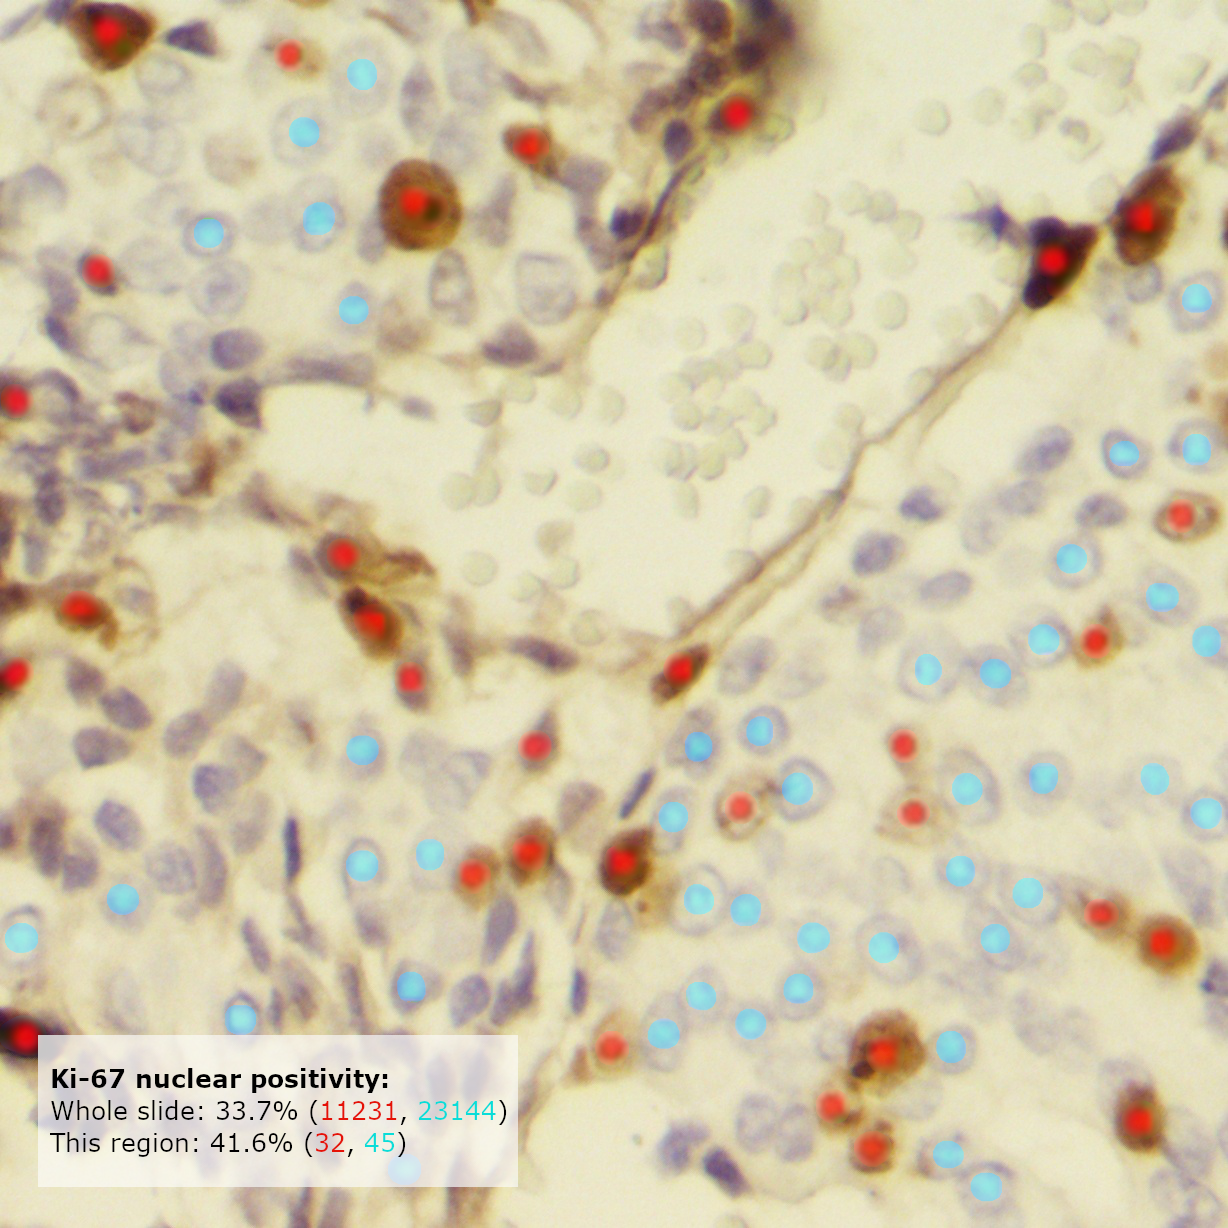
\includegraphics[width=0.85\linewidth]{base_image.png}
    \caption{The sample AI output showing nucleus annotations and overall Ki-67 quantification result.}
    \label{fig:exampleoutput}
\end{figure}

\subsubsection{Selection and Creation of Example Explanation}

In the main body of the questionnaire, respondents were presented with the sample output of a fictitious AI solution for assistance in detection and grading of Ki-67 nuclear positivity,  shown in Figure~\ref{fig:exampleoutput}. Each questionnaire page displayed an alternative example explanation of the sample AI output, with each explanation falling into one of five main classes representing the state of the art described in Section~\ref{sec:related:classes}.

Given their relative ease of implementation, \textbf{Saliency Map} examples were generated using real techniques from the state of the art, applied on the PathoNet model with Neuroscope~\cite{schorr_neuroscope_2021}, an xAI toolbox for deep learning-based segmentation models. The techniques used were guided backpropagation~\cite{springenberg2014striving} and Grad-CAM~\cite{selvaraju2017grad} with respect to the class output layer of the model. The Grad-CAM implementations were presented as both global (an overlay on the entire input region) and local (an overlay on a single nucleus) explanations. Each participant was shown both a global and local example.

The other explanation classes were mocked up with image processing software, based upon existing or hypothetical explainability approaches from the literature, and guided by feedback from pathologists at the Charité Berlin, as well as ML and medical AI experts at Fraunhofer MEVIS and the Technical University of Berlin.

\textbf{Concept Attribution} examples were constructed based on the TCAV approach of \citet{kim2018interpretability}, such that the relative importance of a set of human-interpretable concepts to the positive model outcomes were displayed as an explanation for the overall AI output. Two variations were included, featuring alternative wording for the high-level concepts. 

\textbf{Prototype} examples featured an inset image showing two nuclei that were marked in the Grad-CAM saliency map (as above) as most strongly relevant for the Ki-67 positive and negative classes, respectively.

\textbf{Counterfactual} examples were created based on a generative latent variable traversal approach similar like those of \citet{liu2019generative}. These were supplemented with manually decision boundaries and an additional implementation showing two axes of variation on one figure. The examples themselves were created by morphing between prototypical examples of positive, negative and unclassified nuclei using an open source tool~\cite{diffmorph:github}.

\textbf{Trust Scores} examples were created to represent the concept of per-annotation confidences, grouped into low- and high-confidence classes. These were created by intersecting the class activation Grad-CAM maps with the PathoNet classifications and using the aggregated per-pixel relevance over each nucleus as a proxy for per-annotation model confidence, grouping by value into their respective confidence class.

To better represent the diversity of approaches, a number of example from each class was chosen to approximately reflect its prevalence in the literature. To mitigate the impact of potentially uninformative individual implementations, multiple image variants of selected instances were prepared where practical, with one of these displayed at random for each participant. 

A total number of seven examples to be displayed was chosen to limit the estimated questionnaire completion time to around five minutes. This time limit was chosen to minimise the risk of fatigue and participant dropout, particularly in light of the limited availability of the target audience. To mitigate the impact of primacy and recency, explanation classes were displayed in random order, whilst keeping examples from the same class consecutive. The examples and their variants are shown in Figure~\ref{fig:classes_overview}.

\begin{figure*}
\centering
\begin{minipage}[c]{0.85\textwidth}
    \includegraphics[width=\linewidth]{xAI Classes Overview reordered.png}
    \caption{Explanation examples, along with their plain-text descriptions and image variants, as presented in the online questionnaire and face-to-face interviews. The figure is provided in high resolution and can be zoomed for a detailed view.}
    \label{fig:classes_overview}
\end{minipage}
\end{figure*}

\subsubsection{Rating questions}
 For each explanation, respondents expressed their degree of agreement, rated on a 7-point scale between \textit{Strongly disagree} and \textit{Strongly agree}, to each of four following statements:

 \begin{enumerate}
    \item I find the explanation intuitively understandable
    \item The explanation helps me to understand factors relevant to the algorithm
    \item The explanation helps me to decide whether I can trust the generated annotations
    \item The explanation provides me with valuable information for my work
\end{enumerate}

These statements were designed to gauge a measure of usability, similar to that targeted by the System Usability Scale (SUS)~\cite{brooke1996sus} and the xAI-oriented System Causability Scale (SCS) \cite{HolzingerEtAl:2020:QualityOfExplanations}, in a format appropriate for a short survey with multiple, non-interactive examples. The ordering was chosen to reflect a hierarchy of needs, whereby each subsequent item is unlikely to be highly rated unless there is a strong agreement on all previous statements, with the aim of reducing cognitive load without the need for explicit branching. A sample screenshot of the questionnaire is shown in Figure~\ref{fig:examplepage}.

 \begin{figure*}[ht]
    \centering
    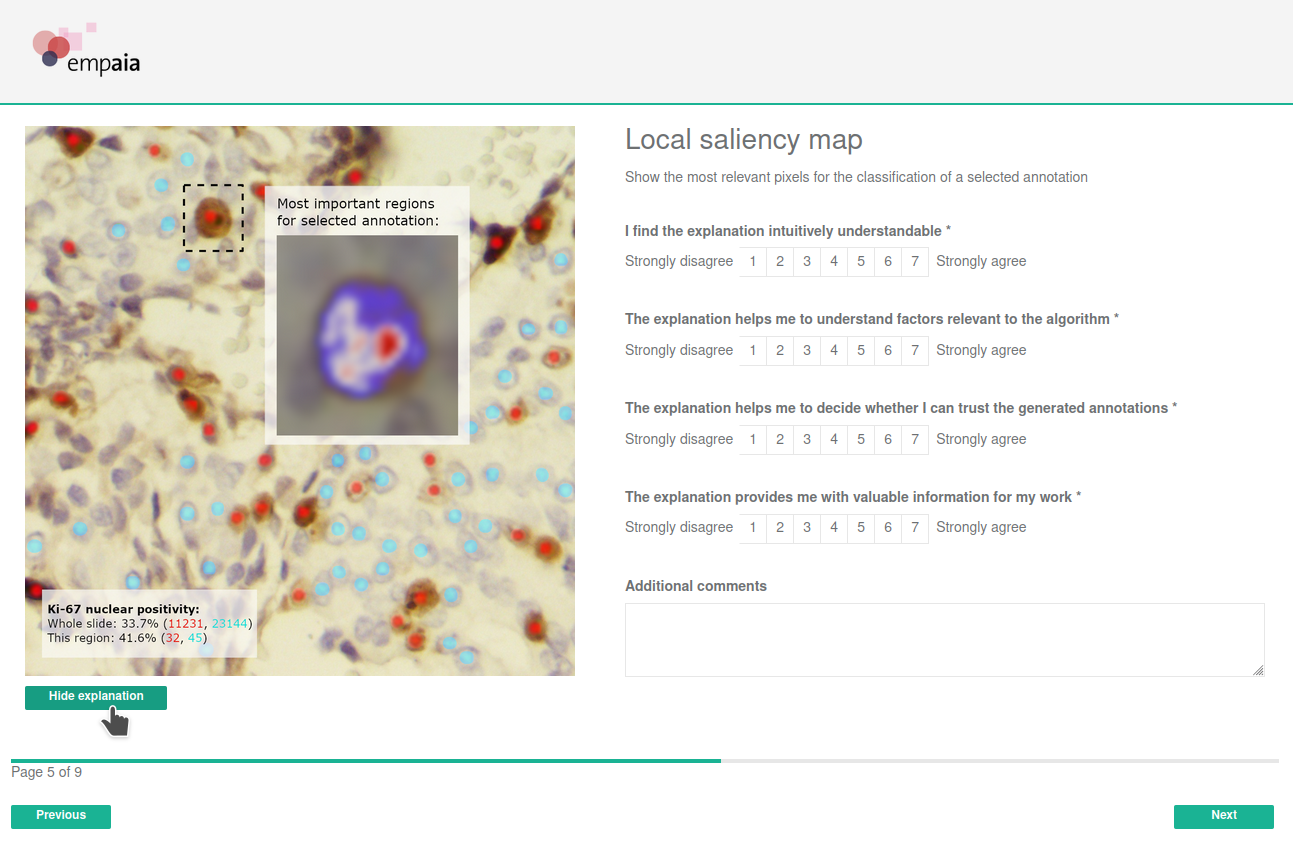
\includegraphics[width=0.75\linewidth]{example_page.png}
    \caption{An example explanation as presented to a participant. The sample AI output is overlaid with one of the possible explanation instances. Clicking on either the image or the \emph{Hide/Show explanation} toggles visibility of the explanation for A/B comparison. Each explanation is accompanied by a name and short plain-text description. The four Likert statements are shown on the right, with an optional comments field below.}
    \label{fig:examplepage}
 \end{figure*}
 
\subsubsection{User profiling}

The following information about each respondent was collected:

\begin{itemize}
    \setlength\itemsep{1pt}
    \item Age
    \item Professional position
    \item Usage of digital pathology or telepathology
    \item Usage of AI solutions
    \item Familiarity with technical details of machine learning
    \item Familiarity with AI applications in pathology
\end{itemize}

These questions closely follow those posed in a user-profiling questionnaire to pathologists disseminated by the Medical University of Graz \cite{HolzingerEtAl:2021:PersonasToolbox}, to allow for cross-evaluation of these results in future work.

\subsubsection{Dissemination strategy}

The questionnaire was open to submissions between 11.06.2021 -- 26.07.2021, having been made public via Twitter on 11.06.2021 (@TheEMPAIA) and again on 15.07.2021 (@DAI\_Labor) and via the EMPAIA newsletter (14.07.2021).

\subsection{Expert interview design}
\label{sec:interviewdesign}
Expert interviews were conducted over video call with a semi-structured format, loosely following the structure of the online questionnaire. Following a short introduction to the outline, goals and purposes of the interview, including the collection of informed consent to begin recording, the interviewee was asked a few questions regarding their professional position, background and experience with AI applications in pathology. The interviewee was then shown the sample AI output, followed by the example explanations in a randomized order, in a simplified version of the online questionnaire. Each interview lasted around one hour in total.

For each example, the interview was structured around a number of open-ended research questions: 

\begin{itemize}
    \setlength\itemsep{1pt}
    \item How do you interpret the explanation shown here?
    \item What does the explanation tell you about how the model is reaching this outcome?
    \item How does the explanation affect your trust in the model output?
    \item How might an explanation like this be valuable to you?
    \item What could make this type of explanation better?
    \item Are there other tasks for which this explanation might be equally or better suited?
\end{itemize}

Not every question was asked to every participant, and room was left for open-ended discussion with the possibility of branching off into more general ideas about explainability and AI applications in pathology.

\subsection{Results analysis}

The questionnaire data was processed using Python. The complete notebook and raw data can be found in the accompanying code repository~\cite{Evans_xAI_in_Digital_2022}.

The interviews were conducted via Zoom call, recorded with the participants' informed consent. These recordings were transcribed with the assistance of AI-based service Otter.ai~\cite{otterai-2021}. The recordings and transcripts were manually reviewed and structurally coded according to the explanation classes and guiding interview questions described above.

\section{Results}
\label{sec:results}

\subsection{Questionnaire respondents}

A total of 29 respondents submitted their responses to the online questionnaire. Four responses were discarded due to respondents falling outside of the target user group. The remaining 25 consisted of individuals holding professional roles in pathology or neuropathology, either as consultant (12), researcher (6), pathologist in training (4) or technician (3). 

\subsection{Questionnaire responses}

\begin{figure*}
\centering
\begin{minipage}[c]{0.9\textwidth}
    Trust Scores:
    
    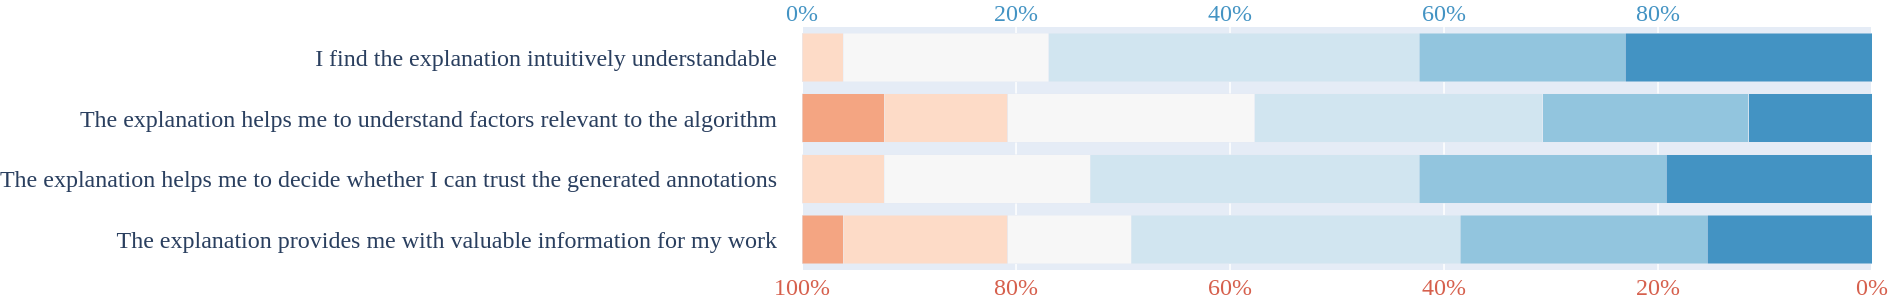
\includegraphics[width=\linewidth]{0_TrustScores.png}
    
    Counterfactuals (One-axis):
    
    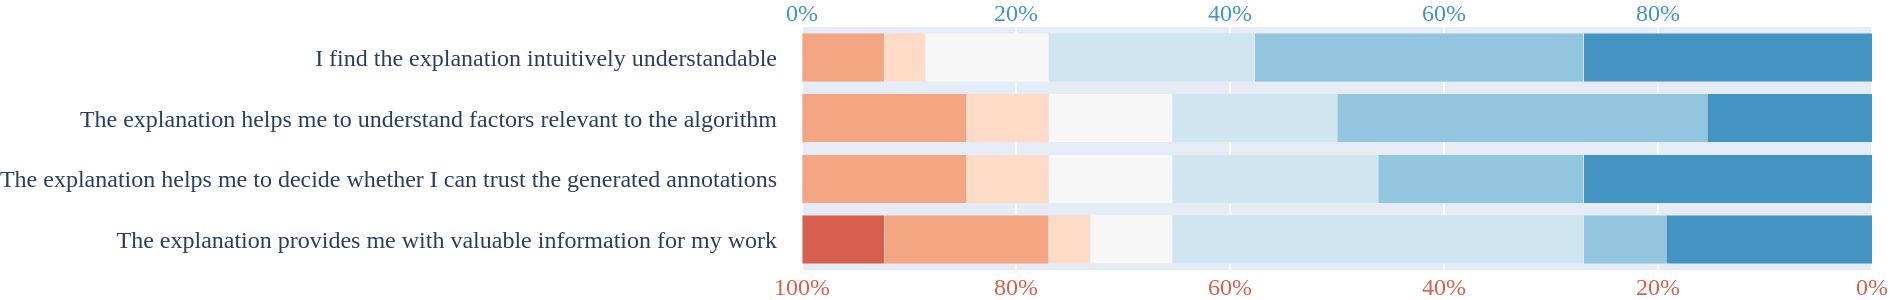
\includegraphics[width=\linewidth]{1_CounterfactualsOneaxis.png}
    
    Concept Attribution:
    
    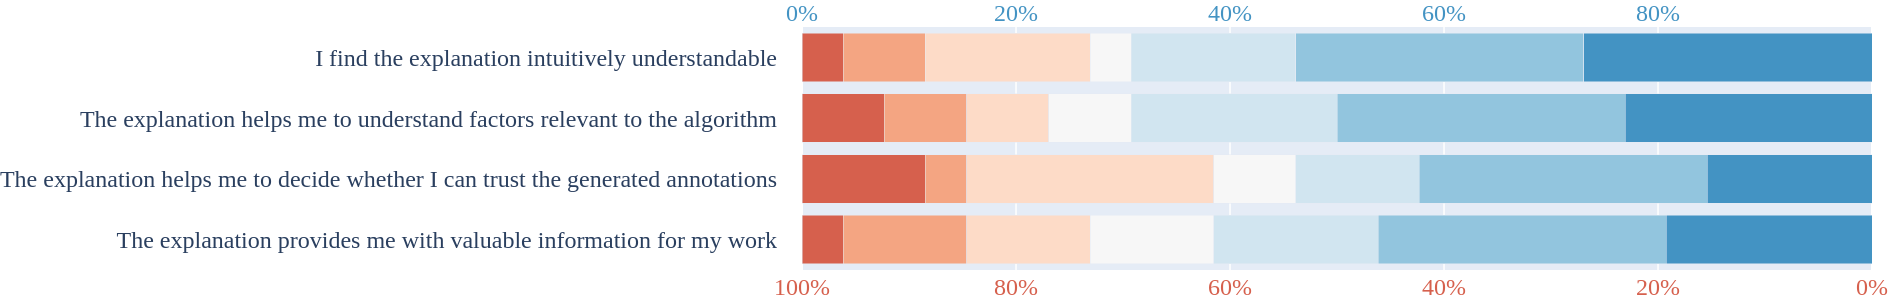
\includegraphics[width=\linewidth]{2_ConceptAttribution.png}
    
    Counterfactuals (Two-axis):
    
    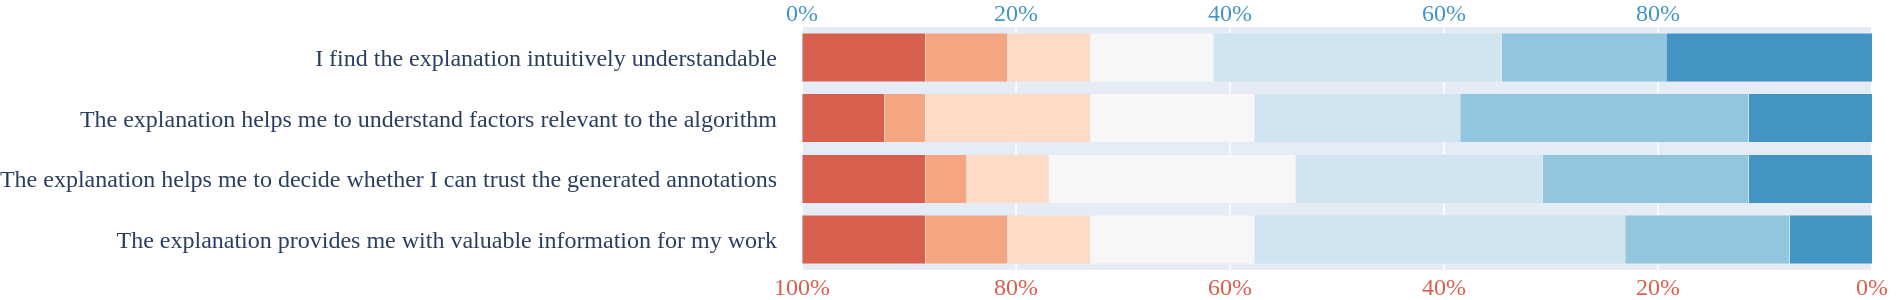
\includegraphics[width=\linewidth]{3_CounterfactualsTwoaxis.png}
    
    Prototypes:
    
    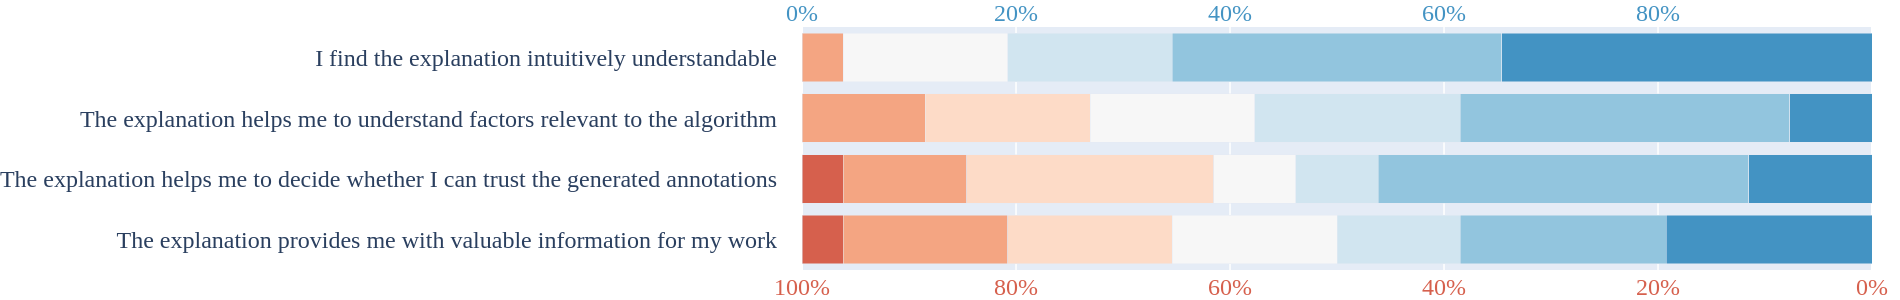
\includegraphics[width=\linewidth]{4_Prototypes.png}
    
    Saliency map (Global):
    
    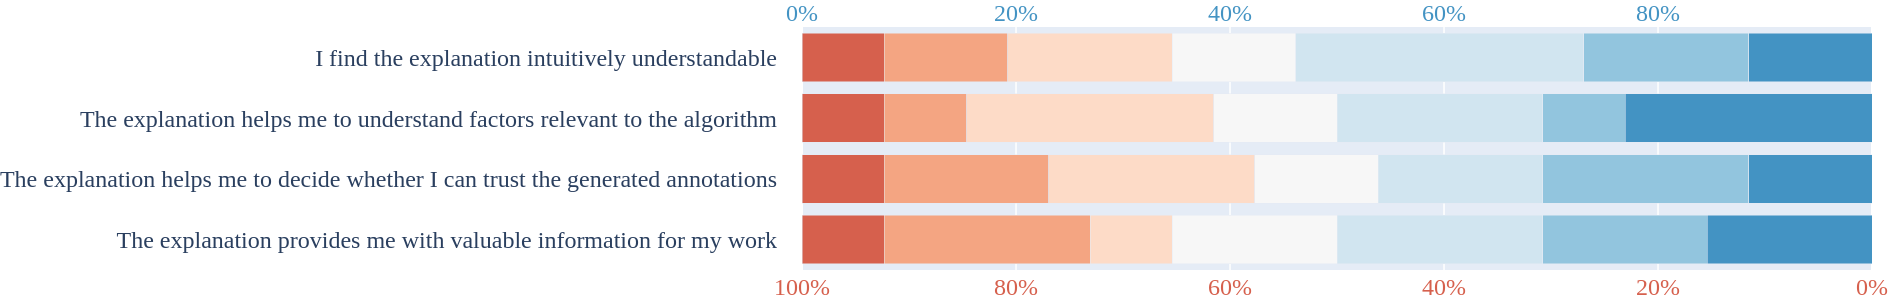
\includegraphics[width=\linewidth]{5_SaliencyMapGlobal.png}
    
    Saliency map (Local):
    
    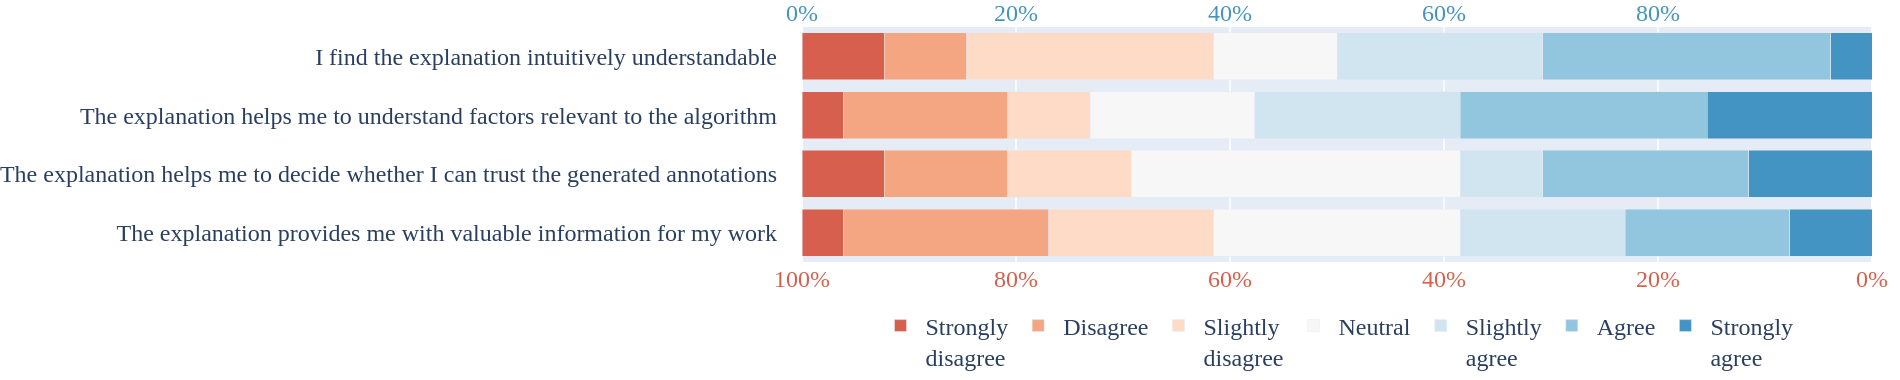
\includegraphics[width=\linewidth]{6_SaliencyMapLocal.png}
    \caption{Distribution of responses from 25 admitted online questionnaire submissions.}
\label{fig:results}
\end{minipage}
\end{figure*}

The results of the online questionnaire are shown in Figure~\ref{fig:results}. Each bar shows the proportion of responses to the four Likert items shown relating to each of the explanation examples shown in Figure~\ref{fig:classes_overview}. Explanation examples are presented in descending order of total positive responses (\textit{slightly agree} to \textit{strongly agree}) to the fourth Likert statement: ``The explanation provides me with valuable information for my work''. Trust scores were the most widely accepted explanation by this metric, while the explanation receiving the most positive median response was the one-axis presentation of counterfactuals.

\subsection{Interview participants}

Six board-certified pathologists (denoted P1--6) participated in video interviews, each lasting around 60 minutes. All interview participants were involved with research in pathology in some capacity, and three were currently involved in routine clinical practice. Years of experience as a certified consultant ranged from one to 45, with one participant being the current director of pathology, another a retired director, at major German research hospitals.

All participants of the interviews were familiar with the field of digital pathology and had some contact with AI applications, both in the research context (P1,\,2,\,5,\,6) and the applied and regulatory context (P3,\,5,\,6). Three participants reported being familiar with AI, but only having limited knowledge of the internal workings of it (P1,\,2,\,5). Furthermore, two participants (P5,\,6) reported having applied AI solutions to routine diagnostic tasks, albeit with unsatisfactory results. P3 and P4 had not seen or completed the questionnaire beforehand; all other participants had.

To protect the anonymity of participants, the video recordings and transcriptions are not made publicly available. Anonymized excerpts from the original transcripts may be made available by request to the corresponding author.

\subsection{Interview findings}

Approximately 360 minutes of interviews were recorded, transcribed and analysed. The resulting findings are presented here, grouped according to topic and explanation class. Comments and observations not directly related to any of the explanation classes described were grouped according to topic and are presented as follows.

\subsubsection{Use of AI in pathology}

It was observed that the term `AI' is vague,  particularly in light of the EU's developing regulatory terminology~\cite{ISO_IEC_22989}; ``Nobody knows what \dots artificial intelligence [is]. Nobody knows what \dots intelligence [is]" (P3). It was noted that, according to such definitions, AI has been applied to pathology for decades in the form of numerical modelling, regression, etc. Similarly, computer-assisted diagnosis has existed in some form or another for many decades, with image processing methods, counters, microscope-mounted cameras, etc. In light of this, the modern trend of deep learning applications to digitized slides was regarded as the logical next step in an ongoing process of innovation (P1,\,3).

AI solutions were often regarded as an extension of technology applied by pathologists for decades, numerical modelling, counters, microscope-mounted cameras, etc., assisting with simple but time-consuming tasks (P1,\,3,\,6); e.g. counting cells or estimating percentages. Speed was often named the highest priority for AI solutions, with the rationale that if the AI did not save the pathologist time, they would simply perform the task themselves (P4--6). The slide digitisation process itself was also named as a limiting factor; i.e., by the time a slide had been scanned and was ready to be viewed digitally and/or processed by an AI solution, the pathologist could have already completed the task under a microscope (P4). It was suggested that slide digitisation needs to reach a critical level of adoption ``over 90\%'' (P6) in order for such applications to make sense.

Two participants expressed the opinion that the pathologist's liability for their decisions, and therefore the obligation to check every result and slide anyway, was limiting the usefulness of AI solutions (P4,\,6). It was suggested that AI solutions could be helpful as a backup, giving a second opinion or flagging features worth reviewing, even after the pathologist has made their own diagnosis. To this effect, the impartiality of AI solutions (for instance, to the seniority of the pathologist) was cited as a strength (P4).

Regarding the state of AI in pathology, limitations regarding accuracy (P5) and data protection (P6) were cited as prohibitive for the use of commercial solutions in clinical settings. It was observed that ``you cannot [just] buy it at the App Store" (P3), rather than machine learning techniques must become part of pathologist's training in order for AI to be effectively applied to pathology, and that the lack of mutual understanding between computer scientists and pathologists was a major factor limiting adoption (P3,\,5).

The issue of inter-pathologist variability in Ki-67 positivity quantification was identified; ``[It] is very boring to count positive or negative nuclei. And most of these things are now based on estimations only, and therefore the results are very weak .... in breast pathology, there's a threshold of Ki-67 positivity of 14.4\%, for selecting some kinds of patients to get chemotherapy or not, and nobody can [estimate] 14.4\% ... but it is the official recommendation of some bodies in European and national pathology, breast oncology" (P1).

Some participants considered AI assistance to be a useful tool in mitigating this issue (P1--3), citing the ability of AI solutions to work systematically without becoming fatigued (P1,\,3) and the potential for them to make better estimations by taking into account other data modalities; e.g. cell morphology, or molecular data (P2).

Conversely, it was suggested that this task was too trivial for AI assistance to be practical (P6) or that lack of standardized training data represents a prohibitive limitation to their potential accuracy (P3). Another participant identified that the pathologist's fine-tuning of AI parameters (e.g. positivity threshold) would anyway reintroduce the same subjective variability, should they have this option (P2).

\subsubsection{Trust in AI}
\label{sec:trustinAI}
The pathologist's own judgement was cited as the primary basis for judging the accuracy, and therefore trustworthiness, of an AI system (P5,\,6). It was suggested that pathologists' trust in an AI solution would be established after extensive use, testing, and comparison with the work of multiple colleagues (P5).

External validation was commonly identified as a critical prerequisite to trust in an AI solution (P1,\,2,\,4,\,5). It was suggested that AI solutions can and should be subject to more forms of validation than the work of pathologists normally would (P2). Diversity (P1,\,5) and experience (P6) of annotating pathologists were stressed as critical factors in assessing the quality of validation and/or training data. Annotations from three pathologists, preferably all from different institutes, was suggested as a minimum requirement for trustworthy ground truth data (P1,\,5).

Participants expressed a range of attitudes toward relinquishing control of the decision-making process to an AI solution. Most participants expressed openness to an AI solution giving a contradicting result to their own (P1--5), with some identifying benefits in giving an AI solution more control over the decision-making process (P1--4), provided it was shown to be reliable. In contrast, one participant expressed the expectation of always having control over the decision boundary of an AI solution, although suggested that the parameters set by an experienced pathologist might then be used with confidence by one with less experience (P6).

The pathologist's legal accountability for their decisions was explicitly mentioned several times (P4,\,6) and used as a rationale both for (P4) and against (P6) endowing more control to an AI solution. 

\subsubsection{Expectations of explanations}

Participants unanimously expressed a preference for simple, visual explanations; "Pathologists are always looking for visual things, matches thinking. Anything outside this modality is foreign" (P1).  Interactivity was often cited as a desirable (P1,\,3,\,4), with one participant suggesting that all of the explanations shown should only be presented as tools with which to interact and manipulate the AI solution, never as a ``source of truth'' (P6).

All participants at some point expressed that explanations tended to increase trust in the AI solution when they demonstrated it making decisions in a relatable manner; i.e., when ``it matches the way we  think when we see the image" (P1). There was a common tendency for participants to attribute relatable decision-making processes when presented with explanations of the AI result; ``We are testing it like we would another pathologist" (P1).

It was mentioned that it is often challenging for pathologists themselves to explain the factors that were important to their own diagnostic decisions, that there is a certain amount of experience and intuition involved (P1,\,2), and that a lack of standardized descriptive vocabulary is also a limitation (P3). However, it was also pointed out that ``we all have passed some information to other pathologists, otherwise there would not be pathologists today" (P1). The method described by one participant for explaining their own decisions would be multi-modal: a region of interest, simply annotated, coupled with high-magnification insets to highlight key features (P6).

% Over the course of the interviews, participants suggested several potential approaches to explain or augment AI solutions for pathology. 

Several participants described variations on the theme of structured annotations (in the style of synoptic reporting) for the slides in question, providing additional context with which to evaluate and confirm the AI output (P2,\,5,\,6). For instance, allow a pathologist to quickly compare descriptors for regions marked by an AI solution as healthy vs. unhealthy (P6). It was implied that these annotations could be automatically generated, either based upon a body of machine-readable ground truth data (P6) or by combining the results of many other feature detection algorithms (P2). 

Automated anomaly detection was also mentioned, wherein an AI solution might -- either as or supplementary to, some other diagnostic output -- flag up features that are statistically rare and/or out of distribution for their training data for manual review (P4,\,5).

An approach was suggested, wherein an AI solution could ``explain'' its decision by showing the images from training data that were most important for a given outcome, comparing this process to that of a pathologist referring to previous cases and reference material to justify their decisions (P1).

In addition to explanations of AI outputs, it was suggested that a ``brochure" containing important information about a given solution would be desirable for building trust it in. Suggested content included: the size of the training dataset, sources of annotations (in particular -- affliations, qualifications and number of expert annotators), corresponding molecular data, and accessible explanations of the methods (e.g. machine learning architectures) employed (P5). 

\subsubsection{Saliency maps}

The reaction of interview participants to the two saliency map examples ranged from difficult to understand, distracting and/or confusing (P1,\,2,\,5) to trivially understandable but not at all useful (P6). Some participants found the explanation interesting but did not know exactly what to interpret from it (P4,\,5). One participant pointed out that it was unclear what was meant by 'the most relevant pixels' (P6).

Many participants identified factors important to the AI solution based on the pixels highlighted as most relevant, including presence, staining, size, and position of the nucleolus, or the staining pattern within the nucleus (P2,\,3,\,5,\,6). It was also pointed out that the explanation was ambiguous: it was not possible to infer which of these different factors were actually important or implied by the explanation (P2,\,5,\,6).

While it was indicated that the congruence between their understanding of what parts of the image are important with those highlighted by the saliency map would help them decide whether to trust the output (P3), most participants did not see this as a meaningful means of establishing the trustworthiness of the AI output (P1,\,2,\,4--6). It was pointed out to be confusing and/or distracting when saliency map and annotations did not align (P4) and redundant when they did; i.e., not understanding “what is output and what is explanation” (P1). 

The majority of participants did not find this type of explanation valuable to them at all for this task (P1,\,2,\,4--6). Even for those who thought it had some value in explaining the factors important to the AI solution, the modality was too detailed and/or too time-consuming (P4--6). Some thought that it might be useful in research (P4) or as just one component in an xAI toolkit (P3).

It was suggested that this form of explanation may be more suitable for classification tasks, where spatial features are more important than for the Ki-67 quantification case (P1,\,2,\,4,\,5). For instance, in the case where the output of an AI solution is the classification of a tumor over a large region. It was suggested that a pathologist could be more likely to trust a solution if the salient regions indicated match their expectations (P1,\,3).

The risk for positive confirmation bias with such explanations was also pointed out. ``[It] is hiding a lot of information. But it's very tempting, because it's very simple", in particular for pathologists not familiar with techniques with which they are generated or at least aware of the many different ways available for doing so (P1). It was suggested that this type of explanation should only be used as one element within an array of explanations or as a final check (P1,\,3).

\subsubsection{Concept attribution}

This example was widely considered intuitively understandable and informative about the factors important for the AI output, albeit with limited value ascribed to this information (P1,\,2,\,4--6). Despite this ambivalent response, some pointed out that it would instill trust the AI output anyway (P2,\,6); i.e. that ``seeing the same factors that I find important makes me more confident in using the information that is provided, if I know that the application uses the same information that I would, as a human being. And applying the procedures that you are applying" (P6). 

% This sentiment was reinforced by the questionnaire results, where 68\% of respondents agreed that the explanation was intuitively understandable (statement 1), with a weak rank correlation between this and its perceived value to the user (\(\rho = 0.38\)). 

It was suggested that this explanation has some value as a sanity check, making clear whether a critical factor is being `missed' by the AI solution. However, in both cases, it was also pointed out that such sanity checks should hopefully be redundant once a pathologist was working with a well-validated, clinically approved solution (P1,\,4).

Criticisms of the explanation were the lack of precision and/or descriptiveness (P1--3) that having to read text is generally undesirable in the pathologist workflow (P3,\,4) -- i.e., that ``a picture is worth more than a thousand words" (P3) -- or that it is simply unsuitable with the task of Ki-67 quantification (P2,\,4--6). 

It was pointed out that the explanation does not describe \textit{how} these factors affect the results, where the thresholds are, or how you would have to change them in order to get a different result (P1,\,6). A comparison was drawn between how a pathologist would explain what was important to them using descriptive language and that this falls short of that level of precision (P1).

Nonetheless, it was suggested that the explanation method is fundamentally promising and could be valuable with refinements (P2--6). Suggested improvements included showing factors in combinations (P2) and/or with finer granularity (P6), or moreover, with indications of thresholds and visual examples demonstrating how these changing factors affect output (P2,\,6), or in combination with an interactive tool for changing these thresholds (P6). 

It was suggested that this type of explanation may be more suitable for other diagnostic tasks; for example, in tasks involving differentiation between metastases and lymphocytes in lymph node sections, where other factors such as cell size and regularity are more important than in the Ki-67 quantification case (P2,\,4--6).

While narrative report generation through identification of text attributes was not deemed to be particularly useful (P1,\,5), the use of text-based explanations or descriptors to the generation of synoptic reports was mentioned (P3,\,5,\,6). 
% This is discussed further in section~\ref{sec:otherideas}.

\subsubsection{Prototypes}

The majority of participants found this explanation intuitively understandable~(P1,\,2,\,3,\,6). The explanation was described as “precise, short and understandable, and reflecting the thinking of pathologists” (P3); “Simply understandable for a human being” (P6).

% , with 80\% of the latter agreeing with the first statement to this effect. However, this ease of intelligibility correlated poorly with its perception as being a valuable explanation (\(\rho_{1,4} = 0.31\))

Aside from helping the user to understand the ``perfect positive and negative result" (P1); ``heaven and hell" (P6), many participants also drew conclusions from this explanation about the specific factors that were important to the AI solution. For instance, that the prototypes shown underlined the importance of staining intensity over other factors~(P2,\,6), ``size, shape, structure and color -- these are also the features you would focus on as a pathologist” (P3), or even indicated where the threshold between positive and negative annotations lay~(P5,\,6). One participant pointed out that the explanation did not explain why cells were detected as tumor cells (P4).

All participants expressed at some point that seeing prototypical examples can help to inform a user's trust in the AI output, with some explaining this with respect to whether they reinforced the idea that the solution was taking into account the same factors as a pathologist~(P1,\,3,\,4,\,6); “you feel better if you understand that the computer is evaluating something that you also do evaluate”~(P6); ``If the [prototype] is not fitting to my understanding [of what it should look like], I know that the result can't be right"~(P4). 

Despite this, there was little consensus that this type of explanation was valuable, with the common criticism that prototypical results do not reflect the diversity that is central to pathology~(P1,\,5,\,6) and/or that the information communicated is too trivial to be useful~(P5). Some participants who identified the explanation as having some value in informing trust in the AI solution later retracted this statement after identifying that the prototypes do not give an indication where the boundary between classifications lies, despite their expectations to the contrary~(P2,\,5); ``If you show me the prototypical positive result, I would expect anything less to be negative" (P5). The risk of positive confirmation bias was pointed out by several participants~(P1,\,2,\,5), leading one participant to name this as ``maybe the worst [explanation]" due to its potential to mislead~(P5).

One participant offered the alternative perspective that having the prototypical results was valuable as an indicator of glass slide quality, more than the quality of the AI output; i.e. if the prototypical examples do not match the pathologist's expectations, it can indicate that there is an issue with the slide preparation and staining (P4).

Several participants suggesting, either implicitly or explicitly, that a counterfactual-based explanation would be a more practical extension of this type of explanation~(P1--3,\,5,\,6), either citing the examples presented or describing their own variation on this theme. One participant suggested that it was helpful to have both types of explanation together, with the implied option of being able to switch between them (P3).

It was suggested that this type of explanation may be more suitable for tasks involving automatic detection of several similarly-presenting cell types, distinguishable only at high magnification (e.g. lymphocytes and plasma cells). In this case, having the prototypical examples of each cell type could give the user confidence that the AI solution  correctly resolved the different cell types without the need for laborious manual inspection (P1).

\subsubsection{Counterfactuals}

All interview participants indicated to some degree or another that the one-axis variant is immediately understandable; ``within a fraction of a second, I can see whether I agree with this or not" (P5); ``Immediately I know why half of the (negative) cells are missing" (P1); with many indicating that the two-axis explanation was not as clear as, or potentially more confusing than the simpler variant (P2--5). 

Interviewed pathologists were almost unanimous in their agreement that the explanation ``helps me understand what the algorithm is looking for” (P1), going so far as to claim that ``this is enough to understand [the result]" (P3). All participants drew some concrete conclusions about the factors important to the AI solution, finding it self-explanatory that staining was the most important factor distinguishing positive nuclei from those marked negative, with some identifying other important factors such as shape, size of nuclei, particularly in separating the positively annotated from the unclassified nuclei (in the two-axis example) (P1--3).

The ability to clearly see the boundary between positively and negatively annotated nuclei was widely considered as an important aid to trusting the AI output for the specific task of quantifying Ki-67 positivity of cancer cells. It was noted that there is another aspect to this task, in deciding which of the nuclei in the slide belong to tumor vs. non-tumor cells. 
Some indicated that the two-axis variant helped them to trust that the solution was making this distinction based on the right factors (P3), or at least, was having the same difficulties in making this distinction that they would (P1,\,5). One participant also suggested that this is not an issue, as the recognition of tumor vs. non-tumor cells is a separate upstream task that would have already been completed by this point ``Once I'm at IHC, I'm just looking at positive or negative''~(P5).

There was a consensus amongst participants that these explanations, or at least the one-axis variant, were a valuable method for understanding and knowing whether to trust the AI output for this particular task. Referring to the two-axis variant, one participant stated, “I think ... this one is the one that provides me all the information I need to assess the results that the algorithm is giving me, based on my own way of accessing [this task], and the pitfalls that I know are there ... because it's also all the information that I use on my own" (P1); another ``I know [artefacts] aren’t being included in the decision because they aren’t shown in the explanation"~(P3). 

Many participants noted that the one-axis case could be more useful due to its simplicity (P2--5), a sentiment backed up by the questionnaire results, in which the two-axis variant rated significantly lower on Q1.

Aside from this, other pitfalls were noted by participants. It was not self-explanatory that the intermediate images were synthetic (P2) and it was not clear which other factors apart from staining intensity were changing between the positive and negative cases in either variant~(P2,\,3). It was also suggested that the explanation could be distracting, causing a pathologist to spend too long scrutinising the exact position of the decision boundary shown in the explanation, at the expense of looking at the slide itself~(P4).

It was suggested that the explanation could be improved by showing an ensemble of counterfactuals to try and explore the different factors that are changing between positive and negative~(P2,\,6). It was also suggested that the on-slide control should also be displayed for comparison~(P6).

Many participants mentioned the possibility of interactivity, with one taking it a step further, suggesting that this explanation should only be used as a tool to  refine the decision boundaries interactively, not as a source of explanation in itself~(P6). Along these lines, they also suggested that this would be a valuable tool for refining multi-modal decision boundaries, e.g. in HER2 grading where, unlike Ki-67, the intensity of staining identified as positive has clinical implications.

\subsubsection{Trust scores}

The labelling of annotations as high- or low-confidence was regarded as being intuitively understandable. Aside from identifying the AI solution's confidence in its annotations, many participants also inferred from this the factors that may have been important to the solution, linking low-confidence annotations to the presence or absence of certain features (P1--3,\,6); e.g. ``[I] can see from this that the staining intensity was important, but the size was not'' (P6).

% , a sentiment corroborated by 76\% of the survey respondents (see Figure~\ref{fig:results}), even as being described as ``almost too basic [to be considered an explanation]'' (P5). % TODO: decide whether this is how we want to use the questionnaire results.

All interview participants indicated that seeing the confidence of annotations (or at least, those that were low confidence) helped them decide whether to trust the results. On the one hand, this stemmed from the implied ability to choose what to do with these low-confidence annotations, e.g. to accept, discard or manually change them (P1--5) or to further refine parameters and thresholds (P6). On the other hand, the coincidence between annotations that were labelled low-confidence and those that the pathologist would also ``have difficulties with" (P1) also increased trust in the AI solution (P1,\,2,\,5,\,6). One participant explained this in terms of giving them the feeling that the AI solution was ``doing the same things that I do" (P2). 

Overall, being able to see the low-confidence annotations was deemed valuable by all participants to assess the AI output, particularly in conjunction with other explanation methods (P4--6), or as a final check before deciding whether to accept the results (P6). Some expressed this in stronger terms ``the way it is presented, I would know at a glance whether I accept this evaluation" (P6); ``[I can] take a glance and say ‘this fits with my interpretation’" (P5). As well as the expectation of the ability to manually resolve low confidence annotations, it was also presumed that this feedback would (or should) train and improve the AI solution (P1,\,6).

In terms of criticism for the approach, it was suggested (P2,\,3) that an effective implementation would require confidence indicators for all classes of annotations. A proposed improvement to the implementation shown would be to display low/high confidence annotations for both positive and negative annotations (P2,\,3); for instance, separately or using different color schemes. 

Aside from confidence scores on a per-annotation basis, information about overall model confidence, including details of validation performance, training data, etc. was identified as an important factor for building trust.

\section{Discussion}
\label{sec:Discussion}

\subsection{Summary}
This paper set out to answer the following research questions:

\researchquestions

To address these questions, we invited pathologists from research and clinical practice to take part in an online questionnaire, along with six semi-structured video interviews. These pathologists were presented with examples from five prominent categories of xAI approach, each having the goal of explaining the result of a sample AI solution. They were then asked to discuss their interpretations and/or rate the perceived usability of each. 

\subsection{Interpretation of findings}

The study context was chosen to be narrow enough to enable a meaningful application-grounded study, whilst provide insights as broadly applicable as possible. It is these overarching findings, relating to general guiding principles for xAI development, upon which the discussion primarily focuses.

Overall, the participants in the study placed a high value on the simplicity of explanation methods. While this could be understood in terms of a general user preferences, it is important to also view this within the context of the pathologists' fast-paced routine work. In this setting, saving time was considered to be the most valuable benefit of AI assistance. Explanations involving complex interface elements, accordingly requiring additional scrutiny and/or training to interpret, may serve to undermine this purpose. The preference for visual explanations can also be seen in this light, with the introduction of different modalities into the primarily visual workflow imposing undesirable additional cognitive load.

With respect to the usability of explanation methods, a broad range of modalities were identified as useful \textit{sanity checks} -- i.e. those flagging instances of the AI doing something ``clearly wrong''. Many situations were identified where it would be straightforward for an explanation to discredit the AI system, for example: 

\begin{itemize}
    \setlength{\itemsep}{1pt}
    \item A saliency map highlighting an irrelevant part of the image
    \item Concept attribution omitting critical diagnostic features
    \item Prototypes strongly deviating from ``textbook'' examples
\end{itemize}

By comparison, explanations providing users with a more nuanced understanding of the decision-making factors of the AI system occupied a small subset of potential implementations. Above all, the acceptability and perceived value of such explanations was determined by the degree to which they allowed the user to infer causal factors in the AI system's decision-making. In particular, there was a greater readiness to place trust in AI systems whose explanations seemed to imply causal decision-making processes that were similar to the users' own.

Moreover, participants showed a clear propensity to ascribe relatable (both human- and pathologist-like) causal reasoning to the AI system in order to try and understand the explanations presented. This was particularly noteworthy in examples that designed with the intent of conveying such casual information. For example, the inference of causal factors determining high and low trust scores was readily used as a basis for perceived trustworthiness of results -- in the vein of ``the AI seemed to have the same difficulties that I would''.

This tendency was recognised by participants as introducing significant risk of bias, particularly as a function of ambiguity or omission of information presented by explanations. This was evident in cases where participants themselves made questionable inferences about the reasoning capabilities of the AI system based on the ambiguous explanation presented. Often, it was only during discussion of these results (if at all) that these errors were identified -- errors that that may have passed unnoticed in a real-world scenario. 

For example:
\begin{itemize}
    \item Saliency maps that highlight diagnostically relevant regions, whilst leaving unclear which features caused those regions to be relevant
    \item Counterfactuals in which multiple features simultaneously change, leaving it ambiguous as to which were truly relevant
\end{itemize}

The tendency for positive confirmation bias was particularly notable when explanations presented information that closely matched -- or at least, did not significantly challenge -- the pathologist's expectations. For example: interpreting a prototype representing features correctly associated with a positive classification to imply that the AI system must be using the correct features to make this assessment. In reality, the prototypical case gives no information about how varied or inclusive this class may be within the decision space of the AI system, or where and based on what features the AI system draws this class boundary.

Another trust-building element in interaction between pathologist and xAI system was the ability to ``get to know'' an AI system: To explore its limitations and quirks, with the expectation that explanation-generating mechanisms should provide an interface for this interaction. This \textit{trial period} was many times identified as an essential component in the building of pathologists' trust in AI systems. 

The flavour of this expected interaction varied with attitude toward the role of AI in diagnostic decision-making. Pathologists displaying an openness to AI systems playing a collaborate, even collegial role, in diagnosis expected explanations that enable them to probe AI capabilities like they would a trainee or colleague. On the other hand, those considering AI assistance more in the way of a ``dumb machine'' tended to treat explainability elements as an interface for manual adjustment and filtering of AI results -- with the pathologist firmly in control. For example, the counterfactual example as a control for setting the positive/negative decision boundary, rather than just a visualisation of it.

This split also reflected attitudes in human versus machine fallibility. The more AI-skeptical considered deviations between human and AI assessments to be cause for rejecting the system. Pathologists with a more AI-optimistic outlook considered conflicting, or even incorrect, AI results to be valuable, if nothing else, to keep them ``on their toes''. In these cases, the AI's indifference toward the experience or seniority of the pathologist was deemed an attractive attribute; one often missing from second opinions provided by human colleagues.

Alongside explainability, the traceability and credibility of data and quality assurance methods used for training and validation was identified as a critical factor for building pathologist trust in AI systems.

\subsection{Implications for xAI research}

Our findings strongly support observations that social and cognitive biases strongly affect human interactions with xAI systems~\cite{miller2019explanation, jussupow2021augmenting}, and that an important aspect of this is the tendency to ascribe human-like traits to xAI systems~\cite{de2017people, miller2019explanation}. This emphasises the importance of designing xAI systems that identify, mitigate, and even take advantage of, such biases and predispositions.

The sources and effects of bias evident in our study support many of the observations and strategies for user-centric xAI systems proposed by \citet{wang_designing_2019}. It should be noted that, while these guidelines are theory-driven, we have reached many of the same conclusions based on purely empirical findings, lending valuable credibility to this prior work.

In addition to the role of explainability in building pathologist trust in AI systems, the need to complement such implementations with model and data transparency was reinforced. The implementation of this suggested by users is reminiscent of the ``model facts" label proposed by \citet{sendak2020presenting}, containing a summary of the model, training and inference methods, validation and performance metrics, as well as purposes and warnings, all presented in standardised and user-accessible language. Beyond these desiderata, pathologists in our study emphasised the importance of understanding sources of model training data, in particular, with regards to the credibility and variety of expert annotators.

Our study was motivated in large part by the predominance of algorithmic (rather than user-centric) approaches to xAI represented in the state of the art~\cite{tjoa_survey_2020, poceviciute_survey_2020, antoniadi2021current}. We agree with the observation of \citet{miller2019explanation} that most of this work ``uses only the researchers' intuition of what constitutes a `good' explanation''.  While studies to identify user requirements for explainability represent a marked improvement on this approach, our findings underline the importance of the extra step taken here: evaluating user interactions with potential xAI approaches directly.

Specifically, our study implies some difficult-to-avoid conflicts that may arise between explainability requirements perceived by user and the potential biases that these are liable to introduce.

\subsubsection{Cognitive load vs. Positive confirmation bias}

The time pressure on pathologists during routine examination places a high burden on AI systems and their explainable counterparts to provide UI elements that introduce minimal cognitive load. Preferences expressed by users in this study were for simple, visual elements, with the simplest explanation candidates (prototypes) being considered the most intuitively understandable, and in many cases, the most readily accepted.

However, our findings demonstrate that every detail omitted from an explanation, whether for the sake of simplicity or due to inherent limitation, is an opportunity for user speculation. That is to say, that any gaps or ambiguities in the information presented to the user are liable to be ``filled in'' according to their own expectations and understanding. This introduces a risk of confirmation bias in explanations that underdetermine the factors important for a model output, and in turn, risks lulling users into a false sense of confidence in the AI system to which they pertain.

This is particularly challenging with respect to the user preference for ``intuitively understandable'' explanations and explainability elements, as these inherently draw upon the prior understanding and associations of the user. As these priors vary user-to-user and case-to-case, there is a degree of uncertainty in exactly what information will be perceived by the user through such explanations. To note here, is that even elements that are not designed as explanations per se may be subject to this caveat.

A case in point: the simple \textit{high / low confidence} trust scores featured in this study were based on pathologist feedback that these classes were accessible due to the inherent analogy to confidence in their own annotations and assessments. The intuitive understandability of such a trust score, based upon an implicit correspondence between these indicators, has the potential to be misleading. While more nuanced approaches exist for generating trust scores that are not based solely on the model's own (biased) assessment of confidence, when presented through a simple and intuitive interface, it is difficult to ensure that the factors that it truly represents align with the hidden priors of the user.

This implies a necessity for xAI approaches that are explicit in the information they convey to the user. A trust score better following this principle might be a aggregation of many different factors, available on demand, where each factor has a clear and interpretable meaning: E.g. the data is out of distribution for the model, the image quality is too low, conflicting features were detected, etc.

\subsubsection{Relatability vs. Anthropomorphism}

The expectation of relatable explanations, that is to say, explanations that represent relatable AI reasoning, presents a similar challenge. By making explanations relatable -- i.e. by ``speaking the language of the user'' -- xAI developers risk implying human-like reasoning of AI systems: An effect observed repeatedly throughout this study. There is a body of research demonstrating the fundamental differences between the way in which human beings and modern machine learning systems process visual information~\cite{geirhos2020shortcut}, meaning that such implications may dangerously misrepresent AI capabilities and limitations.

This emphasises the need for further research into user-friendly xAI approaches that provide useful information about the internal workings of black-box systems, whilst remaining true to their abstract and (currently) statistical nature. The development of such xAI tools goes hand-in-hand with the education of users on the capabilities and limitations of AI systems. While this should be primarily accomplished through good (x)AI design, there is also a strong case for active outreach and training of users (in this case, pathologists) in the fundamental theories and current state of AI/ML applications in their domain.

\subsubsection{Human-computer interaction as first-class citizen}

To date, the state of the art in xAI for image analysis is represented by a large number of algorithmic methods, with saliency map generation by one means or another making up the majority, with many more likely awaiting discovery. As demonstrated in our findings, a broad range of these may be useful for sanity checks for AI results. Indeed, this principle is used as a motivating example for much of the current research landscape~\cite{ribeiro2016trust}. 

At the same time, there is a mounting pressure to ``add'' explainability to AI systems, particularly in sensitive domains like medicine. This generates a risk of explanation-generating methods being applied to AI systems without fully taking into consideration the potential second-order effects described here. In light of this, it is important for AI developers to carefully weigh the benefits against risks of inclusion of explainability elements, To this effect, the development of xAI systems should take place in a tight feedback loop with potential user groups, and that this feedback should be viewed through the critical lens of social and cognitive theories of HCI.

If, through this process, the usefulness and usability of explainability elements cannot be reconciled with the sources of bias they might introduce, it may be an indication that their inclusion is simply inappropriate for the use case at hand. In such cases, our findings suggest that it may be safer to either a) rethink the AI system on a more fundamental level, or b) to exclude explainability altogether and live with the limited transparency of a black-box model, rather than running the risk of misleading users.

\subsection{Limitations}

Due to the limited availability of qualified pathologists to take part in research, particularly those involved in routine diagnostic work, the study was conducted on a small sample of 25 questionnaire respondents and six interview participants, with some overlap between these groups. We suggest that the study's lack of statistical power does not undermine the validity of its qualitative findings. The authors nonetheless acknowledge that some effects demonstrated may be either over- or under-represented due to unsampled variability within the target population. 

This limited participant availability also made it necessary to design the research apparatus with brevity in mind. The sample workflow, AI outputs and xAI elements, were therefore simplified and predominantly static. This deviates significantly from the expected user experience~\cite{Kargl-et-al:2020:PathoWorkflows}; specifically, with respect to the inability to view the non-annotated IHC image, adjacent H\&E layers, and to generally pan and zoom through the slide data. It is likely that this limited participants' ability to effectively evaluate the content and usability of the explainability approaches presented. A future study more closely replicating the pathologist user experience would provide valuable insights, although with an increased cost to the technical implementation and time demands on participants.

Some sources of bias may also be exaggerated within the context chosen for this study. There are relatively few diagnostic factors that play an important role in routine Ki-67 quantification, particularly if identification of the relevant tumor regions has already taken place. By asking participants what information they can infer from the explanations provided, we may have introduced an incentive to read too much into these elements, amplifying the effects observed. Similarly, if explanations provide the user with an inappropriate level of detail for the task at hand, there may be a tendency for users to over-represent their preference for simplicity in UI elements.

With respect to these limitations, we emphasise that the selection and implementation of those xAI methods presented are a reflection of the technical state of the art, as well as the thinking of the machine learning researchers, AI developers and pathologists upon whose feedback they were based. They therefore constitute a representative sample of xAI approaches that may realistically be ``added on'' to AI solutions in order to meet a requirement, whether real or perceived, for explainability. Moreover, their support by prior theoretical work, coupled with the risk of harm if not given their due consideration, make these findings critical points of consideration in xAI development, even if they only represent the worst-case scenario.

\section{Conclusion and Future work}
\label{sec:FutureWork}

In this work, a representative set of xAI approaches to AI-assistance in digital pathology were prepared and then evaluated by a cohort of clinical pathologists. The results of this evaluation are represented in the aggregated responses of 25 online questionnaire responses, combined with the analysis of six hours of expert video interviews. 

To date, there have been no end-user oriented studies of xAI applications in the domain of digital pathology. Aside from extensive reviews of the technical landscape~\cite{yang2021unbox, poceviciute_survey_2020}, first steps have been made in the direction of exploring the explainability needs of medical practitioners~\cite{liao2020questioning,cai2019hello,wang_designing_2019}. The novelty of our approach is in the qualitative evaluation of candidate xAI approaches with real expert end-users. Only through such user- and application-grounded studies can such second-order effects as those demonstrated in our findings be revealed and substantiated with empirical findings.

Namely, the results of this study imply challenging balances to strike between the perceived explainability requirements of AI users and the sources of bias that these may be liable to introduce. On the one hand, our findings demonstrate the preference of pathologists for simple visual explanations that mirror their way of thinking and integrate cleanly with their diagnostic workflow. On the other, they suggest dangers associated with explanations that are overly appealing in their simplicity, or allow for too much ambiguity in their interpretation. 

This is important with regard to the current landscape of xAI research, wherein a large number of algorithmic approaches to adding (post-hoc) explainability to black-box models have been developed, based predominantly on researchers' intuition of what users might need. While these technical contributions are valuable, it is important to carefully consider the implications and second-order effects of integrating such approaches into AI systems as afterthoughts. We rather urge developers that the content, modality and purpose of information communicated through xAI elements be guided by the analysis of use cases and requirements from day one.

Where explainability elements are determined to be a necessary component of AI systems, these should rather be explicit than implicit, even if this conflicts with the preferences of users. Where this conflict cannot be easily resolved, it may be an indicator that a more fundamental review of the AI system, and its interaction with the user, is necessary. Alternatively, or additionally, it may indicate that supplementary training and support for users is required for its safe use.

There is fertile ground for further cross-disciplinary studies of this type. In particular, empirical studies of user interaction with explainability elements embedded into more true-to-life workflow would provide further valuable insights. Elements of such studies in digital pathology might include real AI results, displayed within a fully interactive slide viewer, featuring interactive xAI components. This immersive research environment could be augmented with gaze tracking and bio-monitoring technology in order to collect rich quantitative data on user attention and responses. There are also many opportunities to conduct similar studies in pathology, within the context of representative AI-assisted diagnostic tasks whose level of complexity entails a greater need for explainability than that of Ki-67, e.g. grading of prostate tissue.

Our findings also imply important future work in their application to xAI research and development. Safe and effective forms of xAI will balance usability against the fidelity with which they represent the decision-making processes and capabilities of an AI system. This this end, we suggest two immediate avenues for investigation:

The \textit{parallel} path: Explainability elements based on components of the AI decision-making process that are identified as most closely matching the user's decision-making processes. For example, an neural network-based xAI system in digital pathology might display samples from the training data that are most influential, or at least most similar, to a given model outcome. This is an accessible process for the pathologist, who is accustomed to referring to textbook cases in her work, whilst remaining true to the statistical nature of the machine learning model.

The \textit{orthogonal} path: Explainability elements based upon the components of AI decision-making process identified to have as little in common with human reasoning as possible. Deliberate selection of human-\textit{un}relatable aspects of AI inner workings may help to mitigate the effects described by this study, whilst setting up more realistic (and therefore safer and moresustainable) expectations of AI systems by their users.

This second approach runs the risk of alienating users by emphasising the \textit{otherness} of the AI system, and will likely additional training, support and acclimation for users. However, this be a bitter pill to swallow for a more sustainable long-term xAI strategy. After all, it is precisely these aspects of machine intelligence, the ones that diverge most strongly from human reasoning, that underpin the potential for synergy in human-AI cooperation.

\section*{Acknowledgements}

This work was done in the context of EMPAIA, a project funded by the German Federal Ministry for Economic Affairs and Energy, with funding codes 01MK20002A, 01MK20002C and 01MK20002E. Parts of this work have received funding from the Austrian Research Promotion Agency (FFG) under grant agreement No. 879881 (EMPAIA) and by the Austrian Science Fund (FWF), Project: P-32554 explainable Artificial Intelligence. We thank everyone who supported this work by participating in the anonymous online questionnaire. We express special thanks to Luka Brcic, Rita Carvalho, Gunter Haroske, Iris Piwonski and Tomasz Sołtysiński for their valuable contributions. 

\section*{Declaration of Competing Interest}

The authors declare that they have no conflict of interests and no competing financial interests or personal relationships that could have appeared to influence the work reported in this paper. This work does not raise any ethical issues.

\bibliography{references}

\end{document}